\section{TGGs in action}
\label{sect:TGGs_in_Action}
In this section, we shall export our TGG, implement our new constraint, and get our integration running!
 
\begin{enumerate}
\item[$\blacktriangleright$] Export your metamodels and TGG by choosing ``\texttt{Extensions/\-MOFLON::\-Ecore Addin\-/Export all to Workspace}'' as usual in EA and refreshing your Eclipse Metamodel project to trigger code generation.
\end{enumerate}

If you have done everything right, code generation (not code compilation!) should terminate without any error and the structure of the \texttt{gen} folder in \texttt{LearningBox\-To\-Dictionary\-Integration} should resemble Fig.~\ref{fig:gen_folder}.

\begin{figure}[htbp]
\begin{center}
  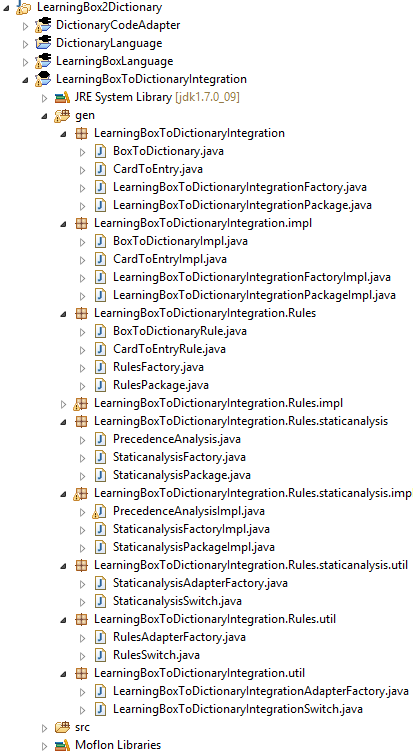
\includegraphics[width=0.7\textwidth]{pics/tggBilder/transformation/tgg22}
  \caption{Integration project after code generation}  
  \label{fig:gen_folder}
\end{center}
\end{figure} 

The Java compilation error in \texttt{Card\-To\-Entry\-Rule\-Impl} is due to our missing \texttt{indexToLevel} implementation, and just means we have to implement the required class by hand.

\begin{enumerate}
\item[$\blacktriangleright$] In \texttt{LearningBox\-To\-Dictionary\-Integration/src} create the Java package \texttt{csp.constraints} and add a new public class \texttt{IndexToLevel}.
\item[$\blacktriangleright$] Implement the class with the code provided in Fig.~\ref{fig:indexToLevel}.
If you take a look at the code it should be pretty clear how the declared adornments are checked and handled appropriately.
With this class, the generated code should now compile without any further errors.
\end{enumerate}

\begin{figure}[htbp]
\begin{center}
  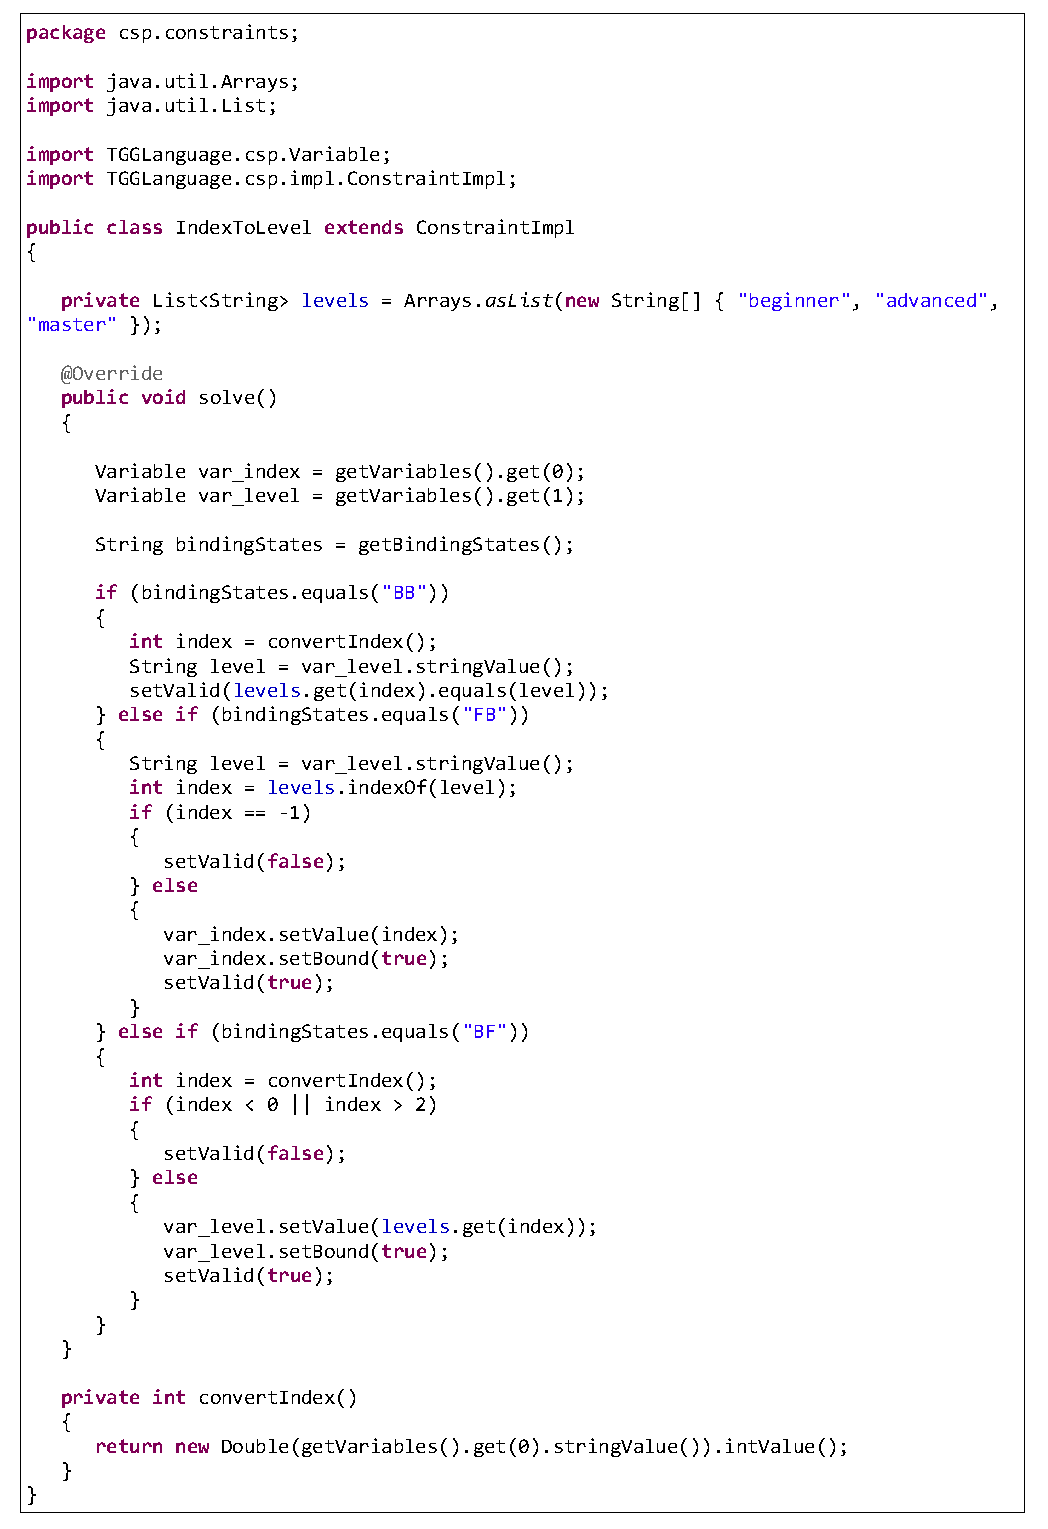
\includegraphics[height=0.64\textheight]{pics/tggBilder/transformation/tgg23}
  \caption{Implementation of our attribute constraint}  
  \label{fig:indexToLevel}
\end{center}
\end{figure} 

In the next few steps, we shall create an instance model\footnote{Refer to Chapter \ref{sect:instance} if you do not know how to do this.} of one of our languages and  transform it to an instance model of the other language according to our TGG, i.e., perform a forward and backward transformation.
As dictionaries are of a much simple structure, let's start with a backward transformation, i.e., dictionary to learning box:

\begin{enumerate}
\item[$\blacktriangleright$] Open \texttt{Dictionary\-Language/model/Dictionary\-Language.ecore} and create a dynamic instance of \texttt{Dictionary}, and save it under \texttt{Learn\-ing\-Box\-To\-Dictionary\-In\-te\-gra\-tion/in\-stan\-ces/Dic\-tion\-ary.xmi} (Fig.~\ref{fig:create_instance_dict}).

\begin{figure}[htbp]
\begin{center}
  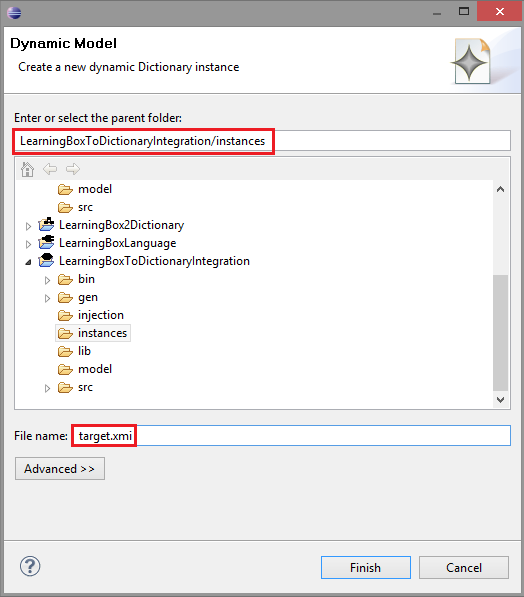
\includegraphics[width=0.7\textwidth]{pics/tggBilder/transformation/tgg24}
  \caption{Create a dynamic instance of \texttt{Dictionary}}  
  \label{fig:create_instance_dict}
\end{center}
\end{figure} 

\item[$\blacktriangleright$] Open \texttt{Dictionary.xmi} and set \texttt{Dictionary.title} to \texttt{English Numbers}. 
\item[$\blacktriangleright$] Create two \texttt{Entry} objects as children of \texttt{Dictionary}: the first entry with \texttt{one : eins} as content and \texttt{beginner} as level, the second with \texttt{eleven : elf} as content and \texttt{advanced} as level (Fig.~\ref{fig:dictionaryxmi}).

\begin{figure}[htbp]
\begin{center}
  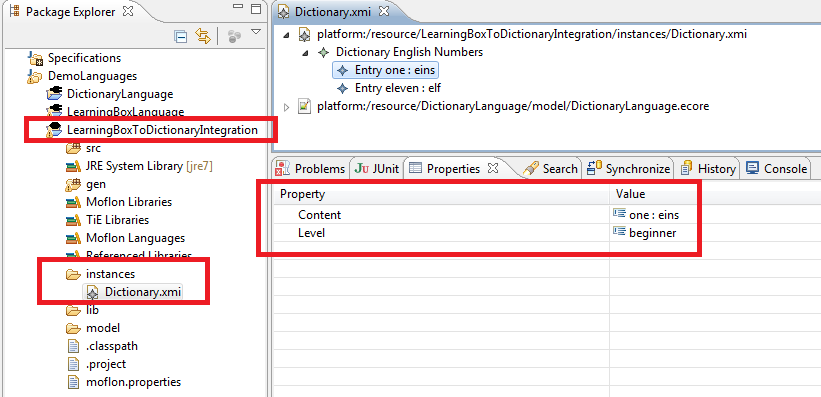
\includegraphics[width=\textwidth]{pics/tggBilder/transformation/tgg26}
  \caption{Contents of the dictionary}  
  \label{fig:dictionaryxmi}
\end{center}
\end{figure} 

\item[$\blacktriangleright$] Create a main class \texttt{TGGMain} in \texttt{LearningBox\-To\-Dictionary\-In\-te\-gra\-tion\-/src} and implement it with the code provided in Fig.~\ref{fig:tggmain}.
\item[$\blacktriangleright$] Run the class and refresh the folder \texttt{LearningBox\-To\-Dictionary\-In\-te\-gra\-tion/\-instances}.
 Check for the created source and correspondence models and open and inspect \texttt{Box.xmi} (Fig~\ref{fig:boxxmi}).

\begin{figure}[htbp]
\begin{center}
  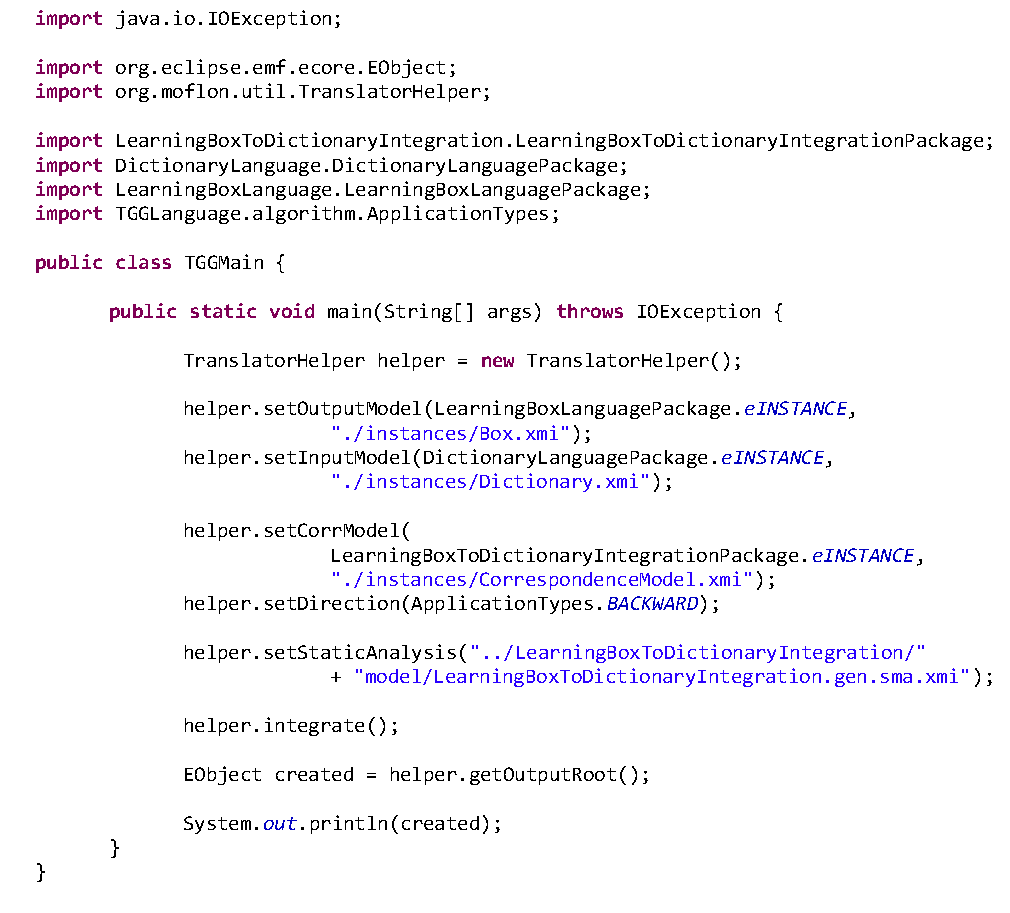
\includegraphics[width=\textwidth]{pics/tggBilder/transformation/tgg25}
  \caption{\texttt{TGGMain} with code to execute a backward transformation}  
  \label{fig:tggmain}
\end{center}
\end{figure} 

\begin{figure}[htbp]
\begin{center}
  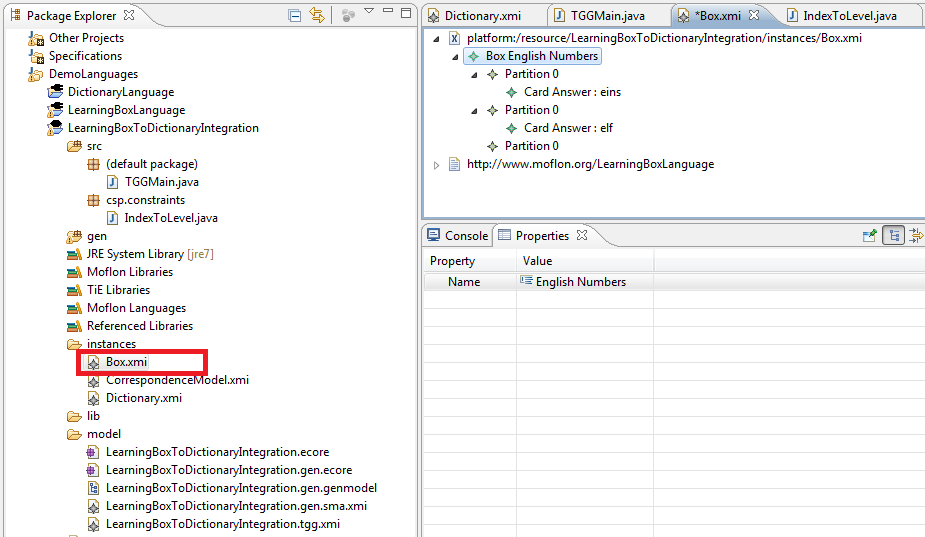
\includegraphics[width=0.9\textwidth]{pics/tggBilder/transformation/tgg27}
  \caption{Generated source model \texttt{Box.xmi}}  
  \label{fig:boxxmi}
\end{center}
\end{figure} 

\end{enumerate}

As you can see, our \texttt{Dictionary} has been backward translated to a \texttt{Box} with the same name (\texttt{English Numbers}), containing three \texttt{Par\-ti\-tions}, as specified in \texttt{Box\-To\-Dictionary\-Rule}.
The two \texttt{Entry} objects have also been translated to \texttt{Card} objects as specified in \texttt{CartToEntryRule}.
Also note that the \texttt{face} and the \texttt{back} of the \texttt{Card}s are consistent with the \texttt{content} of the corresponding \texttt{Entry}, e.g. \texttt{card.face = ``Question : one''} and \texttt{card.back = ``Answer : eins''}. 
The indices of the partitions containing the cards are also consistent with the level of the entry, i.e., \texttt{0} for \texttt{beginner}, and \texttt{1} for \texttt{advanced}.

Congratulations! You have successfully performed your first \emph{backward} transformation from \texttt{Dictionary\-Language} (target model) to \texttt{Learn\-ing\-Box\-Lan\-guage} (source model) using TGGs!

To show that the transformation is actually bidirectional, lets edit the created source model and transform it \emph{forward} to a new target model:

\begin{enumerate}
\item[$\blacktriangleright$] Open \texttt{Box.xmi} and create some new \texttt{Card} objects in the \texttt{Partition}s (e.g., create a new \texttt{Card} with \texttt{Card.face = ``Question : two''}, \texttt{Card.back = ``Answer : zwei''} in \texttt{Partition 0}). 

\item[$\blacktriangleright$] Adjust \texttt{TGGMain.java} carefully as shown in Fig.~\ref{fig:tggmainforward} and run the main method again.

\begin{figure}[htbp]
\begin{center}
  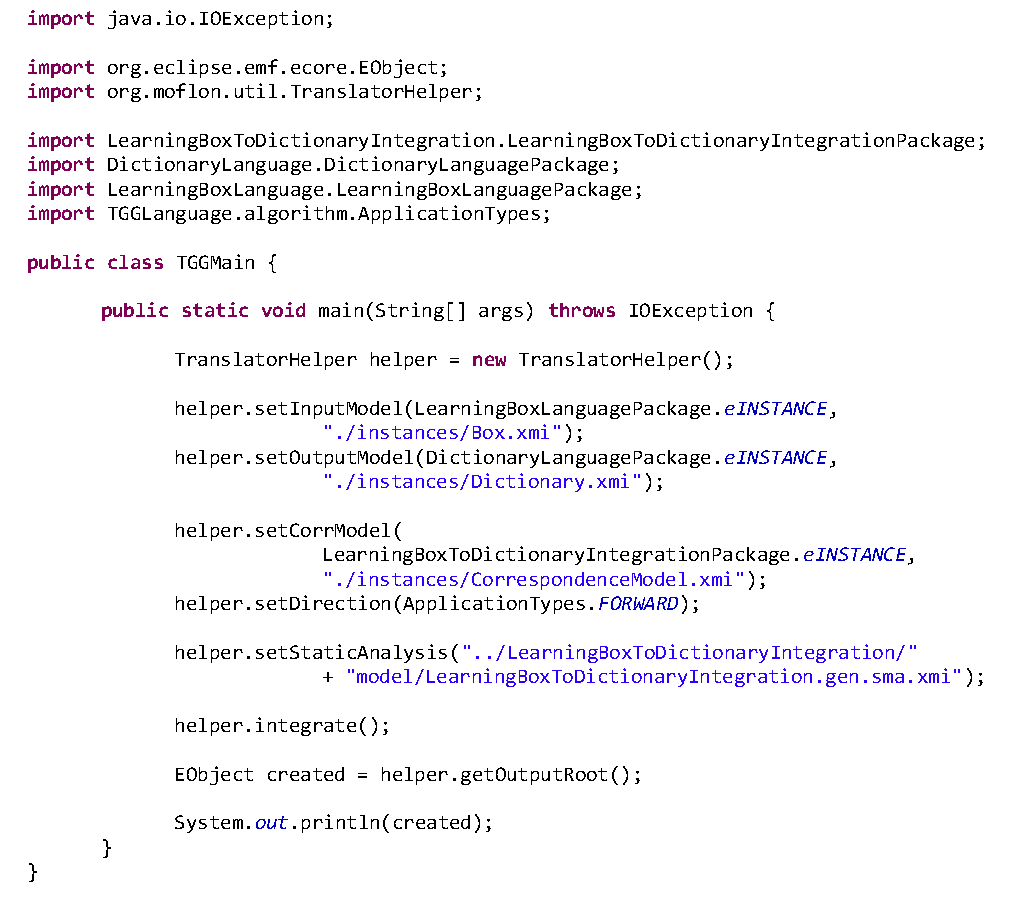
\includegraphics[width=\textwidth]{pics/tggBilder/transformation/tgg28}
  \caption{\texttt{TGGMain} for a \emph{forward} transformation}  
  \label{fig:tggmainforward}
\end{center}
\end{figure} 

\end{enumerate}

If you refresh and inspect \texttt{Dictionary.xmi}, you should be able to see that your new \texttt{Card} objects have been transformed to \texttt{Entry} objects in the dictionary.

To end this chapter on TGGs, lets take a look at a nice \emph{visualization} of the created triple of models:

\begin{enumerate}
\item[$\blacktriangleright$] Right-click the correspondence model \texttt{Correspondence\-Model\-.xmi} and choose \texttt{Start Integrator} from the \texttt{eMoflon} context menu (Fig.~\ref{fig:startintegrator}).
\end{enumerate}

\begin{figure}[htbp]
\begin{center}
  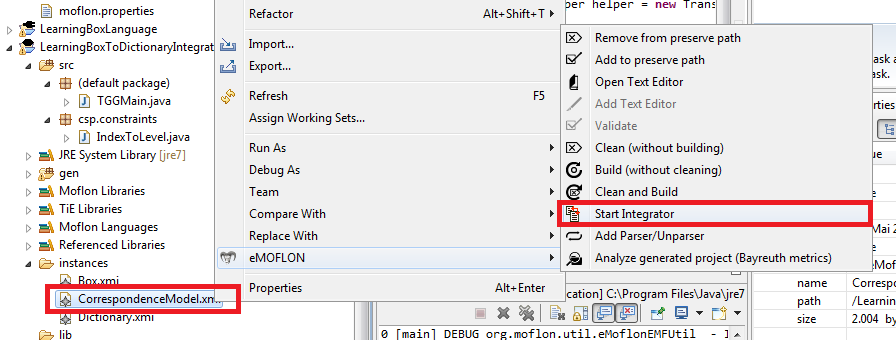
\includegraphics[width=\textwidth]{pics/tggBilder/transformation/tgg29}
  \caption{Starting the integrator}  
  \label{fig:startintegrator}
\end{center}
\end{figure} 

The \emph{eMoflon-Integrator} should be opened visualizing the objects from the source and target models in a treeview with the correspondences between objects depicted as actual ``links" (Fig.~\ref{fig:emoflonintegrator}).
You can implement the \texttt{toString} methods of all classes in the metamodel to improve the visualization.

\begin{figure}[htbp]
\begin{center}
  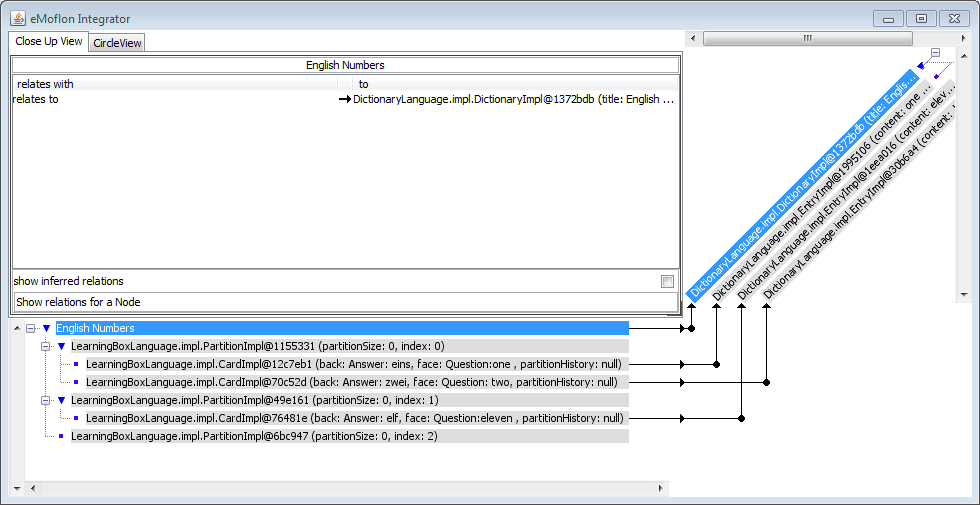
\includegraphics[width=0.9\textwidth]{pics/tggBilder/transformation/tgg30}
  \caption{A visualization of the integration in our integrator}  
  \label{fig:emoflonintegrator}
\end{center}
\end{figure} 

That's it for TGGs for now\ldots 
We hope you enjoyed the short journey! 
Getting used to thinking in TGGs and describing a simultaneous evolution takes some time and patience, but if you feel TGGs could be useful in your domain, then we would be happy to support you as much as we can :)